\begin{figure}

\centering
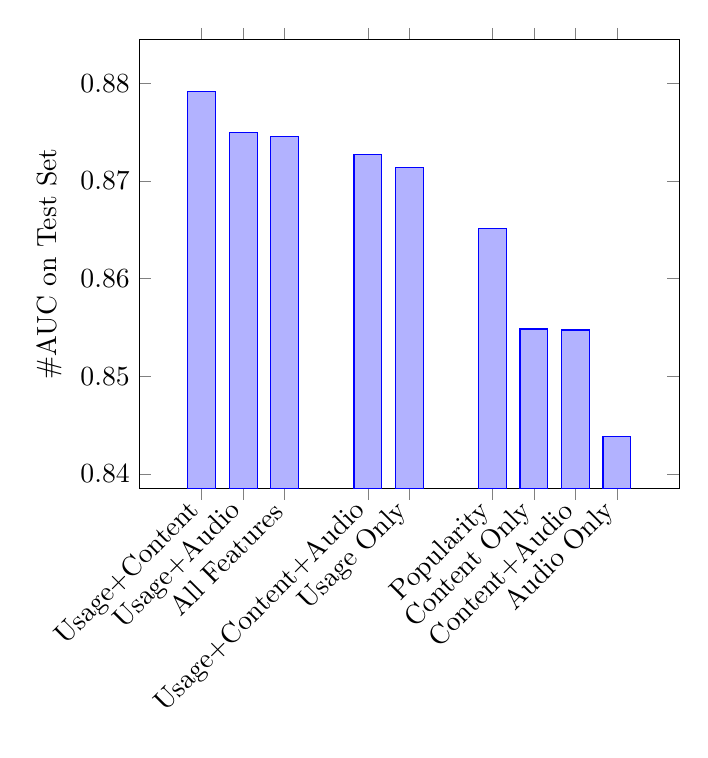
\begin{tikzpicture}
\begin{axis}[ ybar, enlargelimits=0.15, legend style={at={(0.5,-0.15)}, anchor=north,legend columns=-1},
ylabel={\#AUC on Test Set},
symbolic x coords={Usage+Content, Usage+Audio,All Features, ,Usage+Content+Audio, Usage Only, ,Popularity,  Content Only,   Content+Audio,Audio Only},
xtick=data,  nodes near coords align={vertical}, 
x tick label style={rotate=45,anchor=east}
]
 \addplot coordinates {(All Features,0.874533669) (Audio Only,0.843854506)(Content+Audio,0.854736259) (Usage Only, 0.871321339) (Content Only,0.854838861) (Usage+Audio,0.874955404) (Usage+Content,0.879144173)(Popularity,0.865104775)(Usage+Content+Audio,0.872677779)};
 
   \end{axis}
    \end{tikzpicture}
    \caption{Accuracy according to feature group}
    \label{FeaturesFig}
    \end{figure}